\documentclass[noinstructornotes]{ximera}
%handout:  for handout version with no solutions or instructor notes
%handout,instructornotes:  for instructor version with just problems and notes, no solutions
%noinstructornotes:  shows only problem and solutions

%% handout
%% space
%% newpage
%% numbers
%% nooutcomes

%I added the commands here so that I would't have to keep looking them up
%\newcommand{\RR}{\mathbb R}
%\renewcommand{\d}{\,d}
%\newcommand{\dd}[2][]{\frac{d #1}{d #2}}
%\renewcommand{\l}{\ell}
%\newcommand{\ddx}{\frac{d}{dx}}
%\everymath{\displaystyle}
%\newcommand{\dfn}{\textbf}
%\newcommand{\eval}[1]{\bigg[ #1 \bigg]}

%\begin{image}
%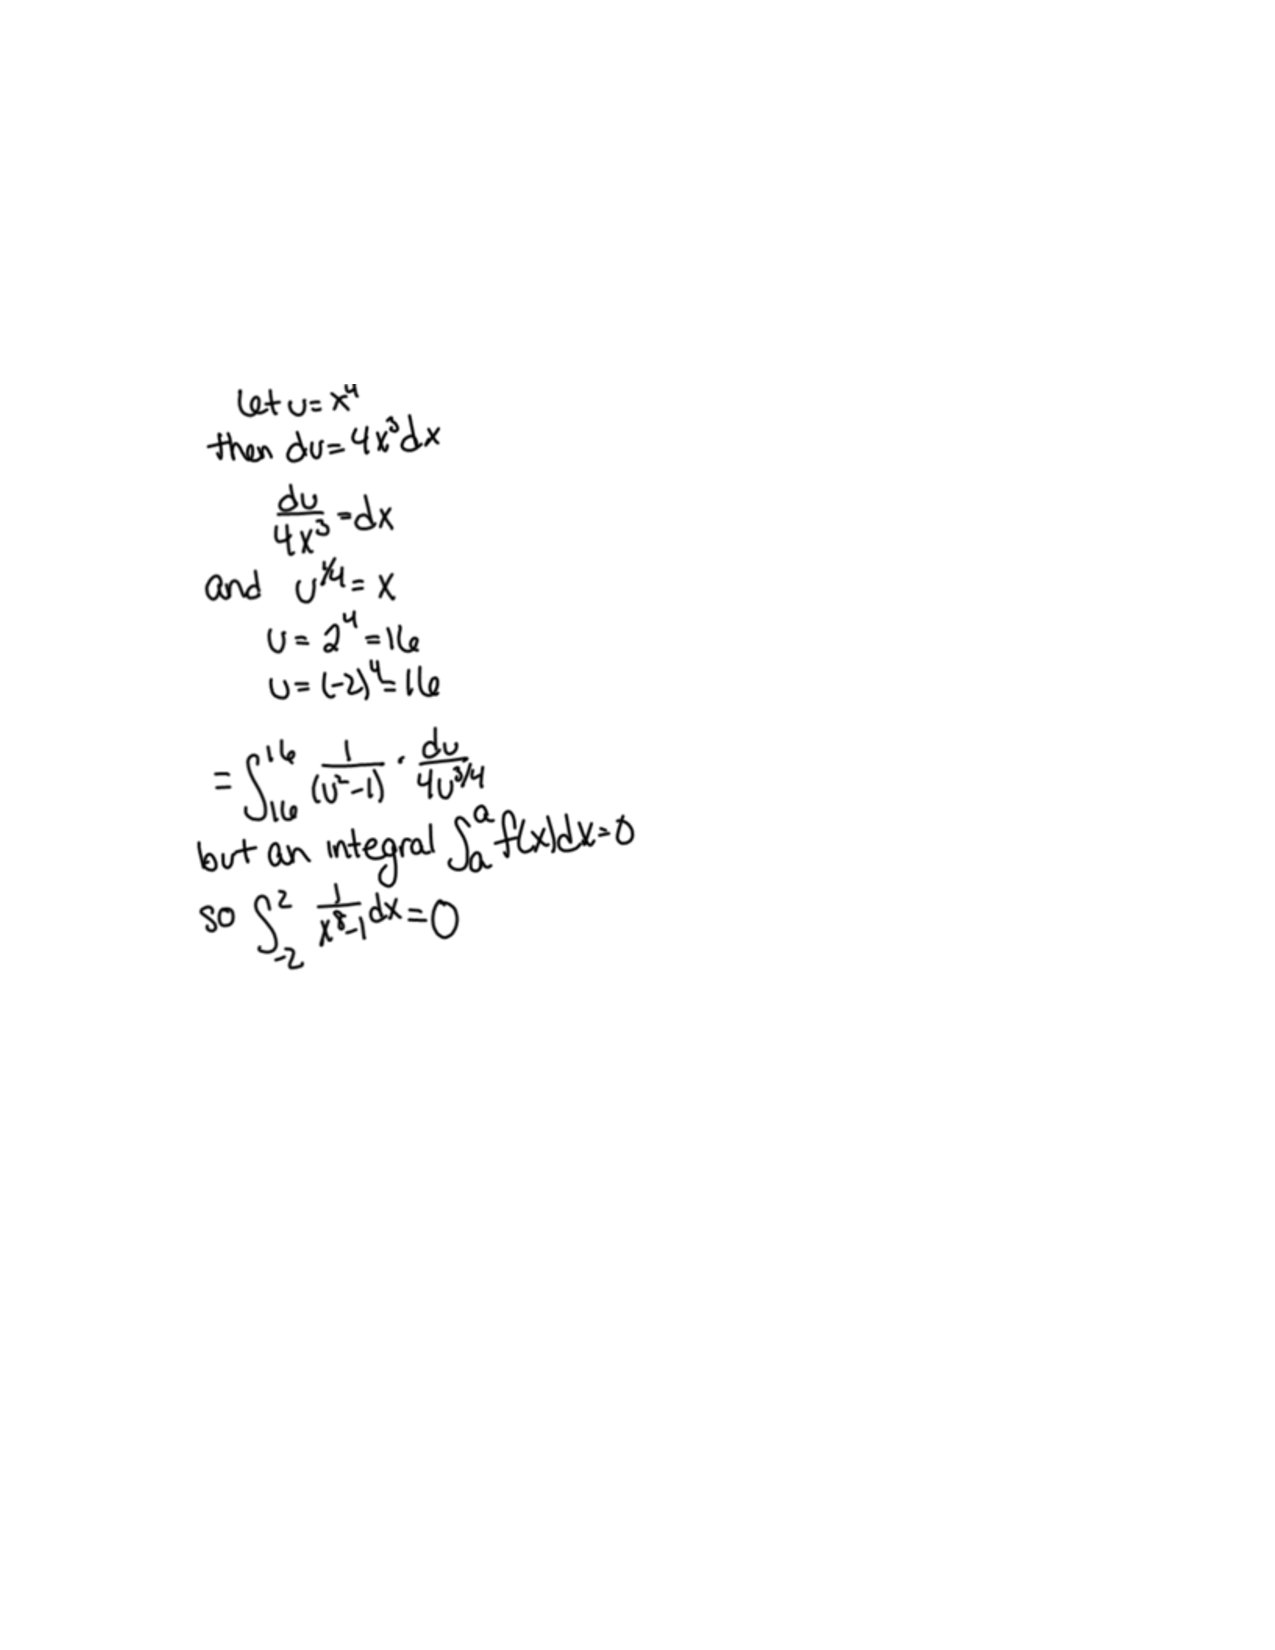
\includegraphics[trim= 170 420 250 180]{Figure1.pdf}
%\end{image}

%add a ``.'' below when used in a specific directory.
\newcommand{\RR}{\mathbb R}
\renewcommand{\d}{\,d}
\newcommand{\dd}[2][]{\frac{d #1}{d #2}}
\renewcommand{\l}{\ell}
\newcommand{\ddx}{\frac{d}{dx}}
\newcommand{\dfn}{\textbf}
\newcommand{\eval}[1]{\bigg[ #1 \bigg]}

\usepackage{multicol}

\renewenvironment{freeResponse}{
\ifhandout\setbox0\vbox\bgroup\else
\begin{trivlist}\item[\hskip \labelsep\bfseries Solution:\hspace{2ex}]
\fi}
{\ifhandout\egroup\else
\end{trivlist}
\fi} %% we can turn off input when making a master document

\title{Recitation \# 3: Volume by Slicing}  

\begin{document}
\begin{abstract}		\end{abstract}
\maketitle



%again, no real warm-up for this section.
\begin{comment}
\section{Warm up:}

	\begin{freeResponse}
	
	\end{freeResponse}
	
\begin{instructorNotes}

\end{instructorNotes}
\end{comment}







\section{Group work:}



%problem 1
\begin{problem}
	\begin{enumerate}
		\item  Consider the region bounded by the curves $y=x^2+8$ and $y=7x-2$.  
		Set up an integral that will compute the volume of the solid whose base is the region and whose cross sections perpendicular to the region and the $x$-axis are:
			\begin{enumerate}
				\item[(i)]  Squares
				\begin{freeResponse}
				We first set the curves equal to each other to see where they intersect
					\begin{align*}
					x^2 + 8 &= 7x - 2  \\
					x^2 - 7x + 10 &= 0  \\
					(x-2)(x-5) &= 0  \\
					x &= 2,5.
					\end{align*}
				By checking the point $x=3$, we see that $7x-2 \geq x^2+8$ over the interval $[2,5]$.  
				So our region is bounded
					\begin{itemize}
					\item  from above by $y=7x-2$
					\item  from below by $y=x^2+8$
					\item  from the left by  $x=2$
					\item  from the right by $x=5$.
					\end{itemize}
								
				The volume of the solid that we are trying to find is given by the integral
				\[
				\int_2^5 A(x) \d x
				\]
				where $A(x)$ is the area of a square (within in the region and perpendicular to the $x$-axis) at a generic point $x$.  
				One side of the square is given by $s(x) = (7x-2) - (x^2+8) = -x^2 + 7x -10$ 
				%(see the picture below).  
				Thus,
				\[
				A(x) = s(x)^2 = (-x^2+7x-10)^2
				\]
				and
				\[
				\text{{\color{red} Volume of region}} = \int_2^5 (-x^2+7x-10)^2 \d x .
				\]
				
					%\begin{image}
					%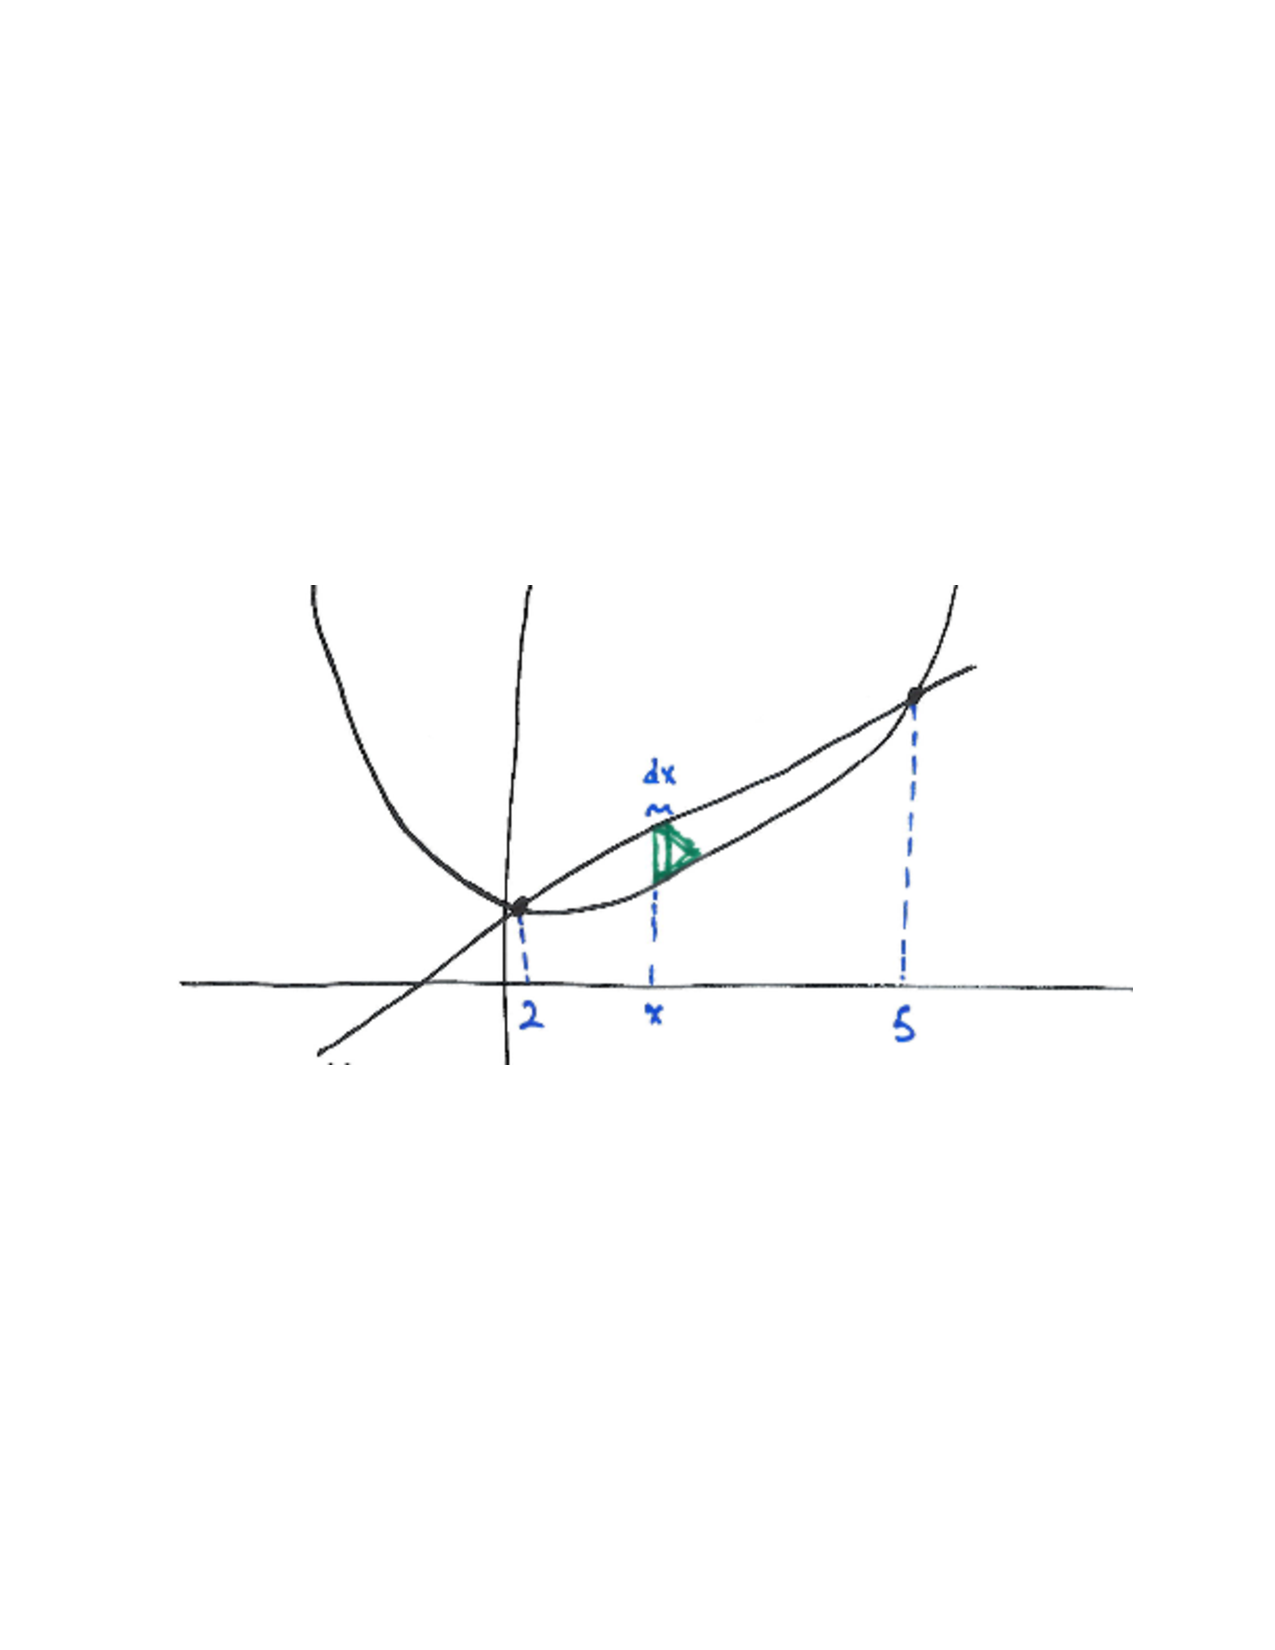
\includegraphics[trim= 240 280 200 270, scale=0.8]{Figure6-3-2.pdf}
					%\end{image}
				\end{freeResponse}
				
				\item[(ii)]  Semicircles
				\begin{freeResponse}
				Everything is exactly the same as in part (a), except now each slice is a semicircle instead of a square.
  
				Recall that the area of half of a circle is $\frac{\pi}{2} r^2$, and at a generic point $x$ the radius satisfies
				\[  
				2r(x) = -x^2+7x-10	\qquad	\Longrightarrow		\qquad	r^2(x) = \frac{1}{4} \left( -x^2+7x-10 \right)^2.
				\]
				Then we have that
					\begin{align*}
					\text{{\color{red} Volume of region}} &= \int_2^5 A(x) \d x  \\
					&= \int_2^5 \frac{\pi}{2} \cdot \frac{1}{4} \left( -x^2+7x-10 \right)^2 \d x  \\
					&= \frac{\pi}{8} \int_2^5 \left( -x^2+7x-10 \right)^2 \d x.
					\end{align*}
				\end{freeResponse}
			\end{enumerate}
		
		\item  Do the same as in (a), except that the solid's cross-sections are perpendicular to the region and the $y$-axis.
		\begin{freeResponse}
			\begin{enumerate}
			\item[(i)] Squares
			
			The structure of this problem is the same as in part (a).  
			We know that the two curves intersect at $x=2,5$, and so plugging those into either equation shows that the $y$-coordinates of these intersection points are $y=12, 33$.  
			Over the region $12 \leq y \leq 33$ we can solve both equations for $x$
				\begin{align*}
				x_1 &= \sqrt{y-8}  \\
				x_2 &= \frac{1}{7} (y+2).
				\end{align*}
			By either checking a point in the interval $[12,33]$ or simply by consulting the picture above, we see that $x_1 \geq x_2$ over this region.  
			Then the slide of a square at a generic point $y$ is
				\[
				s(y) = \sqrt{y-8} - \frac{1}{7}(y+2)
				\]
			and the volume of the region is
				\begin{align*}
				\text{{\color{red} Volume of region}} &= \int_{12}^{33} A(y) \d y  \\
				&= \int_{12}^{33} \left( \sqrt{y-8} - \frac{1}{7}(y+2) \right)^2 \d y.
				\end{align*}
			
			\item[(ii)] Semicircles
			Again, we proceed in exactly the same way as in part (a).  
			From above, we have that
				\[  
				2r(y) = \sqrt{y-8} - \frac{1}{7}(y+2)	\qquad	\Longrightarrow		\qquad	r^2(y) = \frac{1}{4} \left( \sqrt{y-8} - \frac{1}{7}(y+2) \right)^2
				\]
			and
				\begin{align*}
				\text{{\color{red} Volume of region}} &= \int_{12}^{33} A(y) \d y  \\
				&= \int_{12}^{33} \frac{\pi}{2} \cdot \frac{1}{4} \left( \sqrt{y-8} - \frac{1}{7}(y+2) \right)^2 \d y  \\
				&= \frac{\pi}{8} \int_{12}^{33} \left( \sqrt{y-8} - \frac{1}{7}(y+2) \right)^2 \d y.
				\end{align*}
			
			\end{enumerate}
		\end{freeResponse}
	\end{enumerate}
	
\end{problem}

\begin{instructorNotes}
Do 1(a)(i) as a class.  
Have the students do 1(a)(ii) in groups and have a group present.  
Then split the two parts of (b) between the groups.  
Discuss as a class. 
\end{instructorNotes}







%problem 2
\begin{problem}
Set up an integral that will find the volume of the solid formed by revolving the region bounded by the curves $y=x^2-4x+8$ (i.e. $x = 2 \pm \sqrt{y-4}$) and $y=-x^2+10x-12$ (i.e. $x = 5 \pm \sqrt{13-y}$) about:

\begin{image}
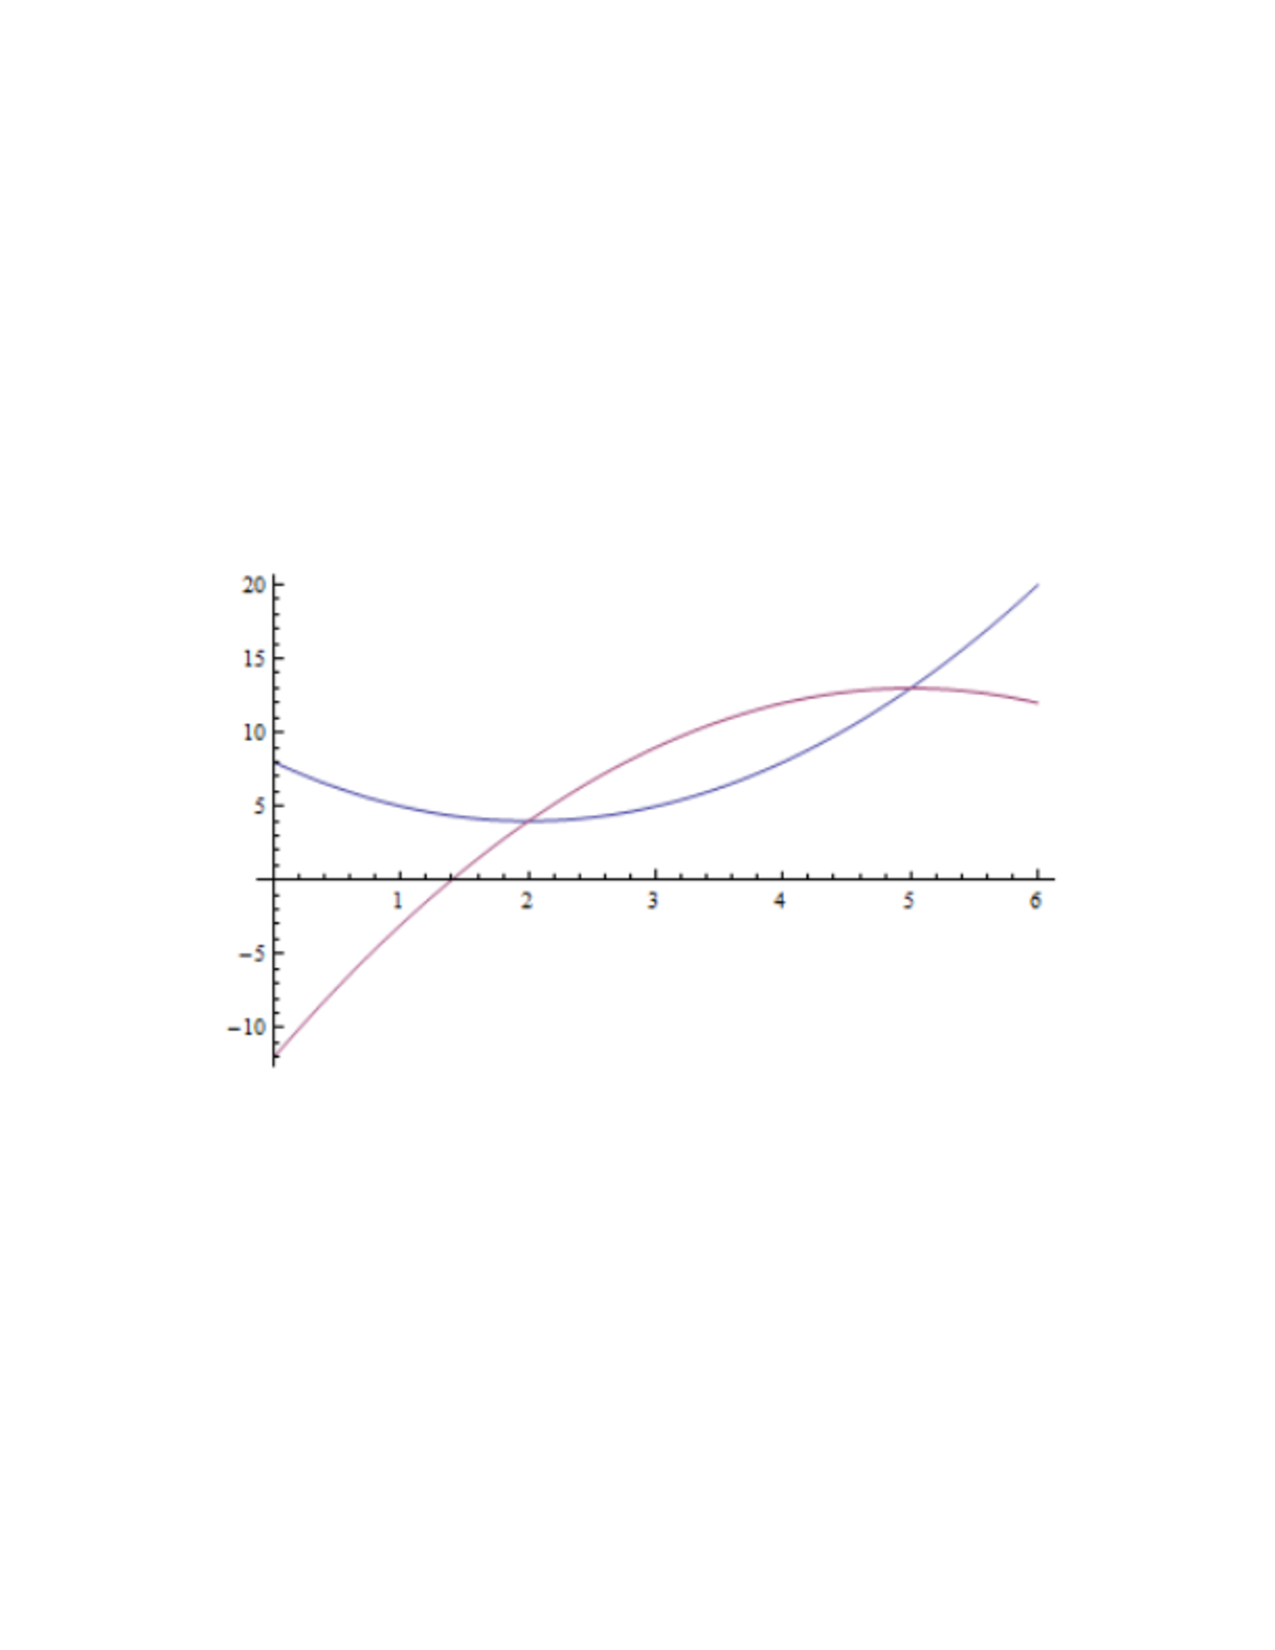
\includegraphics[trim= 240 280 200 270, scale=0.5]{Figure6-3-1.pdf}
\end{image}
	
	\begin{enumerate}
		\item  the $x$-axis
		\begin{freeResponse}
		First, we need to find where the two curves intersect
			\begin{align*}
			x^2-4x+8 &= -x^2+10x-12  \\
			2x^2 -14x +20 &= 0  \\
			x^2 - 7x + 10 &= 0  \\
			(x-2)(x-5) &= 0  \\
			x &= 2,5.
			\end{align*}
		By plugging in the point $x=3$, we see that
			\[
			-x^2+10x-12 \geq x^2-4x+8
			\]
		on the interval $[2,5]$.  
		
		
		
		Notice that a cross section at a generic point $x$ looks like a ``washer".  
		Thus, to find the volume of the surface of revolution, we need to compute
			\[
			\int_2^5 A(x) \d x
			\]
		where $A(x)$ denotes the area of the corresponding washer.  
		Recall that $A(x) = \pi \left( r_{out}^2 - r_{in}^2 \right)$ where $r_{out}$ and $r_{in}$ denote the outside and inside radius of the washer, respectively.  
		
			\begin{image}
		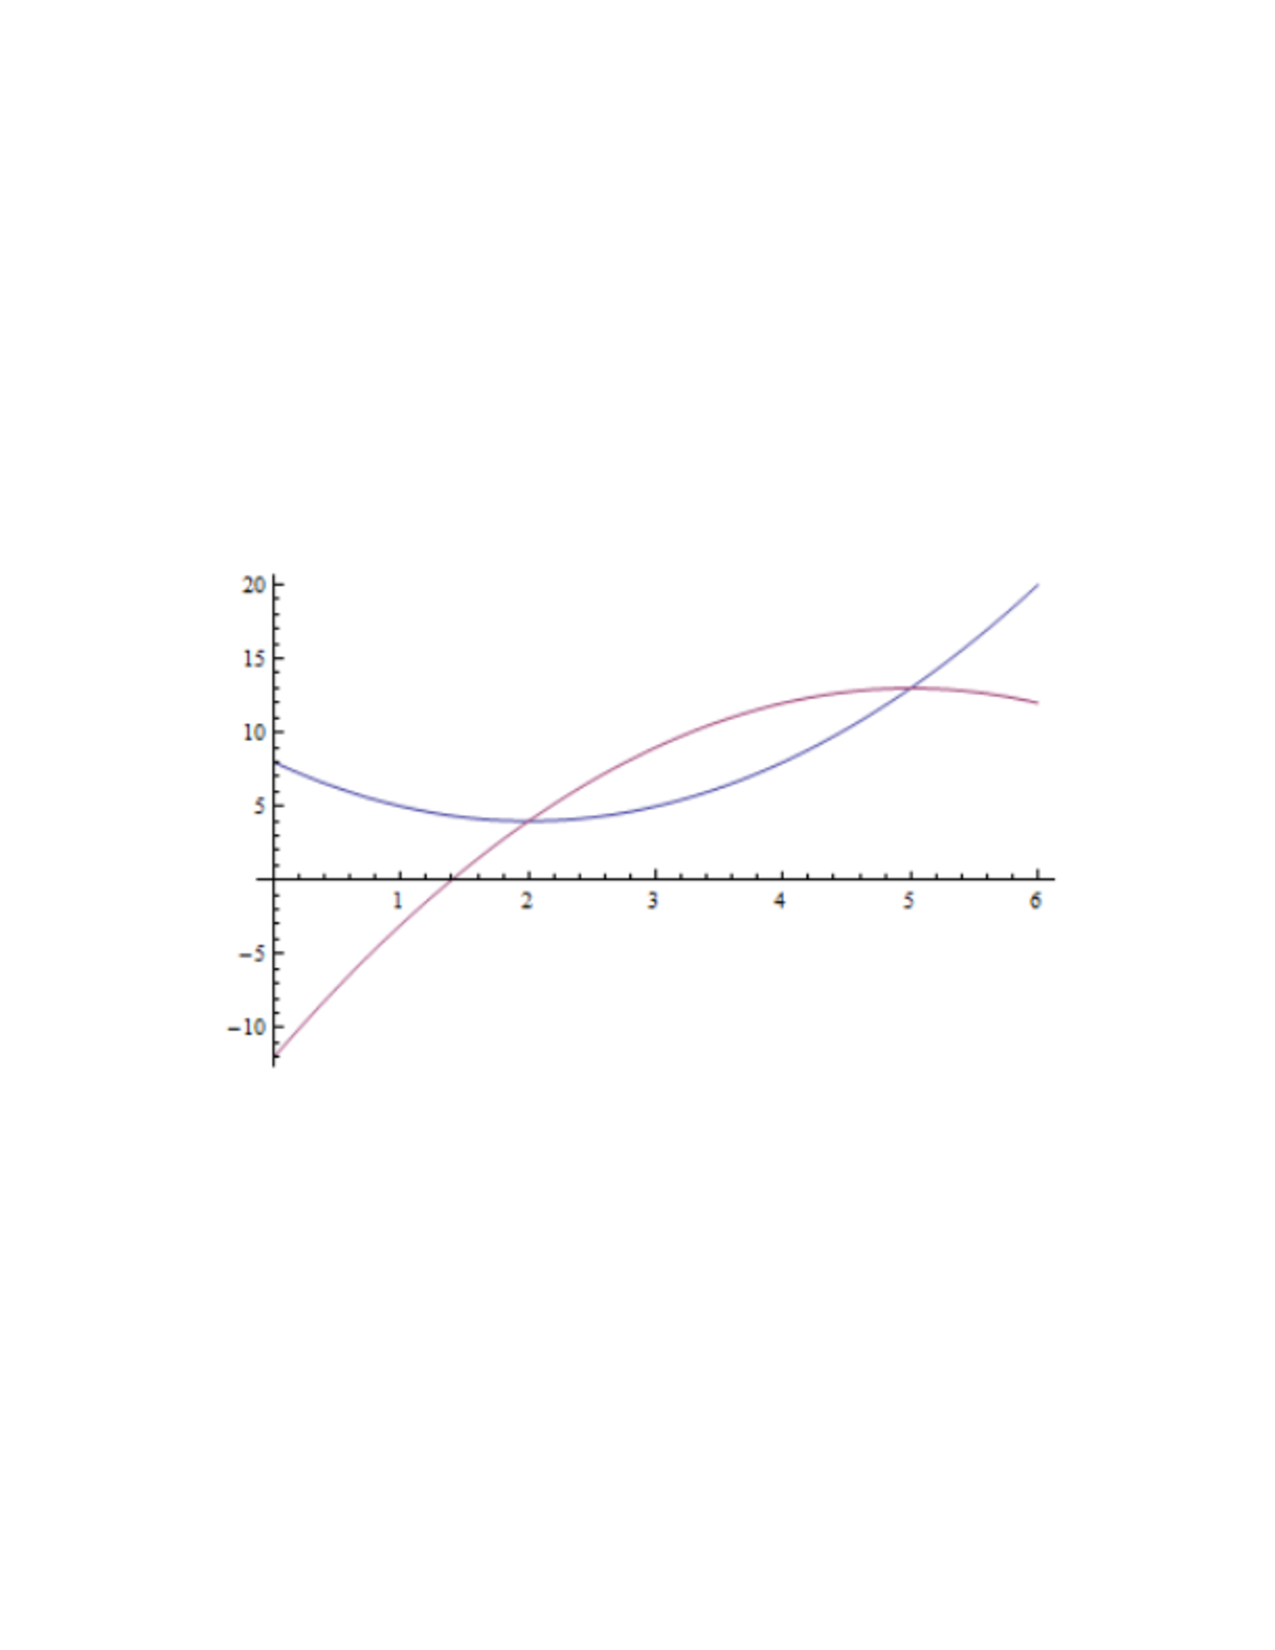
\includegraphics[scale=0.8]{Figure6-3-3new.png}
		\end{image}
		
		Consulting the picture, we see that
			\begin{align*}
			r_{out} = R(x) &= -x^2+10x-12  \\
			r_{in} = r(x) &= x^2-4x+8
			\end{align*}
		and thus
			\[
			\text{{\color{red} Volume of region}} = \pi \int_2^5 \left[ (-x^2+10x-12)^2 - (x^2-4x+8)^2 \right] \d x.
			\]
			
	
		
		%\begin{image}
		%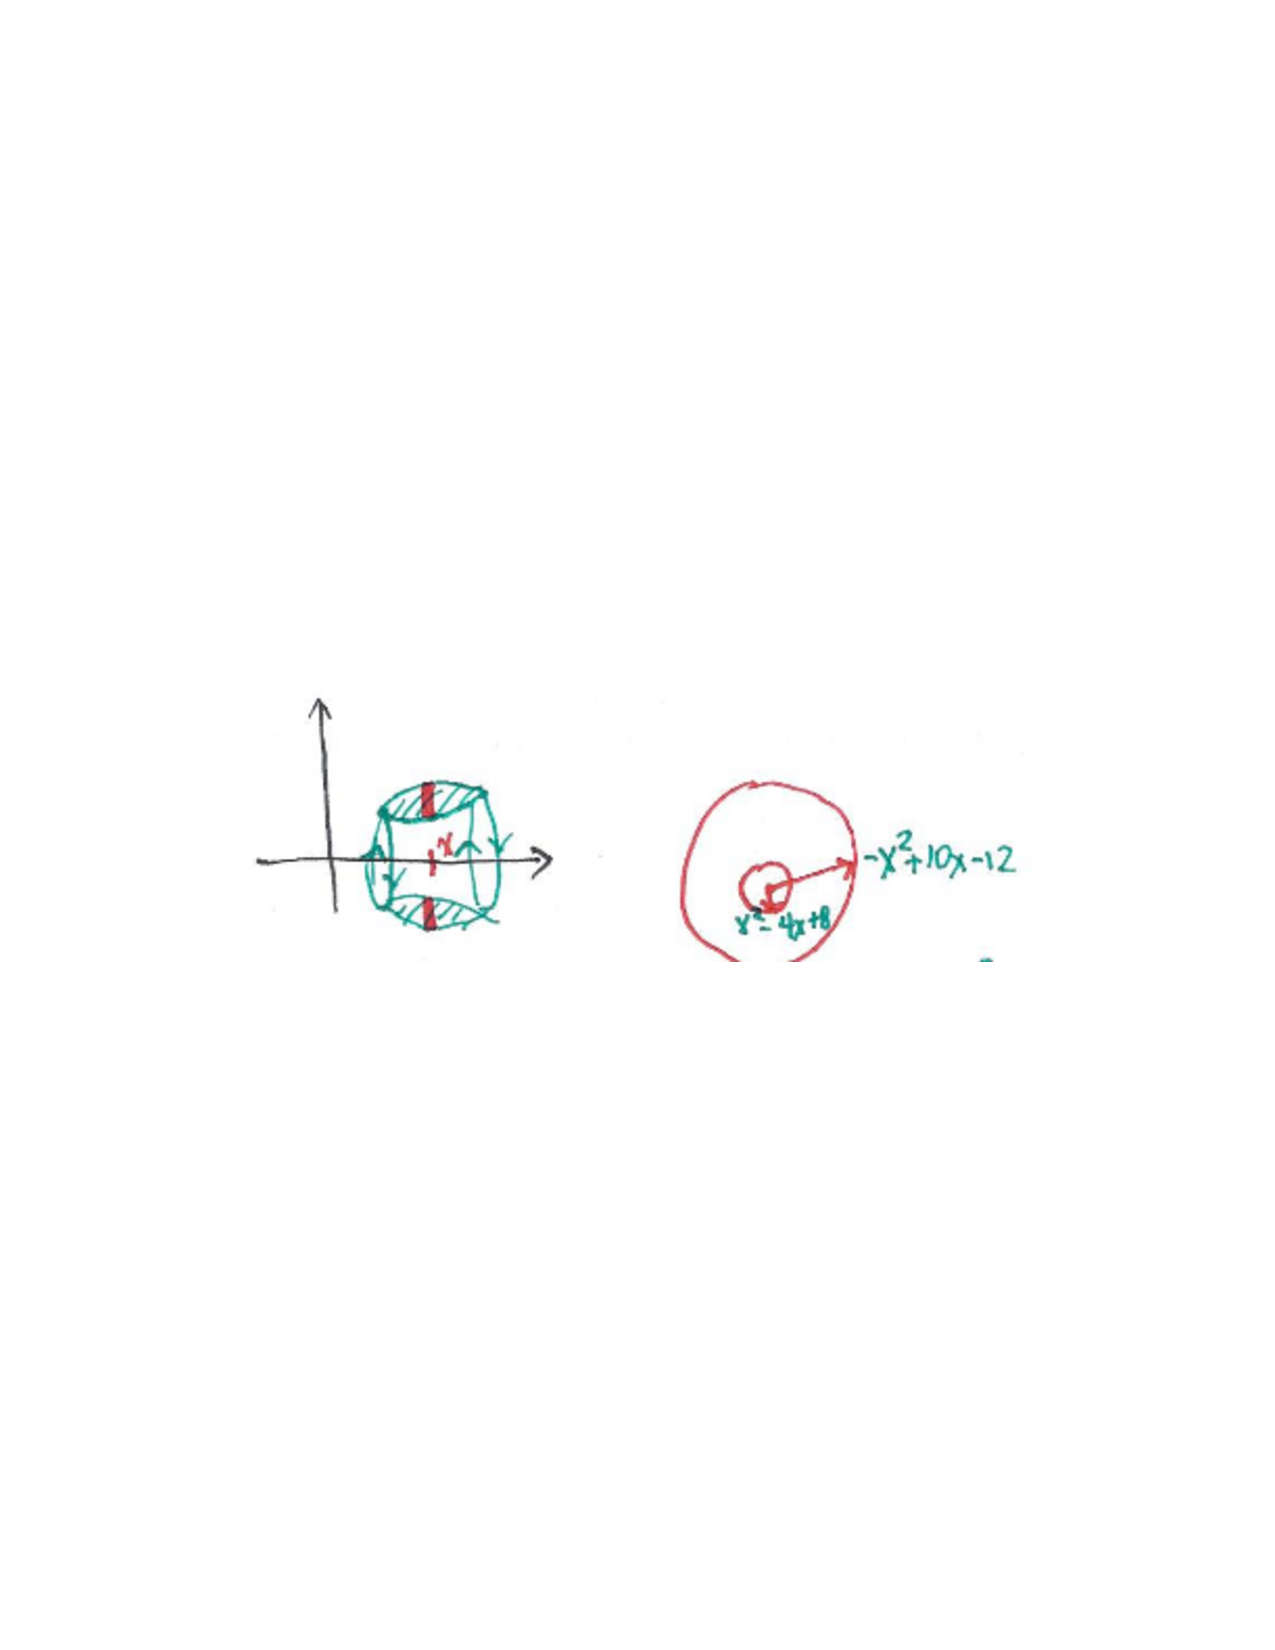
\includegraphics[trim= 240 320 200 330, scale=0.8]{Figure6-3-4.pdf}
		%\end{image}
		\end{freeResponse}
		
		
		
		\item  $y=-3$
		\begin{freeResponse}
		
				\begin{image}
		\includegraphics[scale=0.8]{Figure6-3-5new.png}
		\end{image}
		
		The line $y=-3$ is just the $x$-axis shifted down $3$ units.  
		So both radii just ``grow" by $3$:
			\begin{align*}
			r_{out} = R(x) &= 3 + (-x^2+10x-12) = -x^2 + 10x -9  \\
			r_{in} = r(x) &= 3 + (x^2-4x+8) = x^2 - 4x + 11.
			\end{align*}
		Then
			\[
			\text{{\color{red} Volume of region}} = \pi \int_2^5 \left[ (-x^2+10x-9)^2 - (x^2-4x+11)^2 \right] \d x.
			\]
			

		\end{freeResponse}
		
		
		
		\item  $y=15$
		\begin{freeResponse}
		
		\begin{image}
		\includegraphics[scale=0.8]{Figure6-3-6new.png}
		\end{image}
		
		Now, the line $y=15$ is the $x$-axis shifted up 15 units.  
		This causes a bigger difference than in part (b), since our axis of rotation has moved to the opposite side of the region between the curves.  
		Consulting the picture below, we see that
			\begin{align*}
			r_{out} = R(x) &= 15 - (x^2-4x+8) = -x^2 + 4x + 7  \\
			r_{in} = r(x) &= 15 - (-x^2 + 10x - 12) = x^2 - 10x + 27.
			\end{align*}
		Then
			\[
			\text{{\color{red} Volume of region}} = \pi \int_2^5 \left[ (-x^2+4x+7)^2 - (x^2-10x+27)^2 \right] \d x.
			\]
			
		
		\end{freeResponse}
		
		\item $x=1$
		\begin{freeResponse}
		Now, we are revolving around a vertical line.  Since we need to take slices perpendicular to our axis of rotation, we will now need to integrate in terms of $y$.
		We have the curves $x =2 \pm \sqrt{y-4}$ and $x = 5 \pm \sqrt{13-y}$.  For  $x = 2 \pm \sqrt{y-4}$, we want to take the plus sign because we want the right half of the parabola. 
		For  $x = 5 \pm \sqrt{13-y}$, we wan to take the minus sign because we want the left half of the parabola.
		We also need to calculate the $y$-values of the intersection points.  Let's use the first equation.\\
		$y(2)=(2)^2-4(2)+8 = 4\\
		y(5)=(5)^2-4(5)+8 = 13$
		
				\begin{image}
		\includegraphics[scale=0.8]{Figure6-3-7new.png}
		\end{image}

			\begin{align*}
			r_{out} = R(y) &= (2 + \sqrt{y-4}) - 1 =  1 + \sqrt{y-4}  \\
			r_{in} = r(y) &= (5 - \sqrt{13-y}) - 1 = 4 - \sqrt{13-y} \\
			\end{align*}
		Then
			\[
			\text{{\color{red} Volume of region}} = \pi \int_4^{13} \left[ (1 + \sqrt{y-4})^2 - (4 - \sqrt{13-y})^2 \right] \d y.
			\]
			

	
		\end{freeResponse}
		
		
		\item $x=6$
		
				\begin{image}
		\includegraphics[scale=0.8]{Figure6-3-8new.png}
		\end{image}
		
		\begin{freeResponse}
		This is similar to the previous problem only now the axis is on the other side of the figure.  Recall that horizontal distances are measured as right minus left, so this time we will take the axis minus the curve.

			\begin{align*}
			r_{out} = R(y) &= 6 - (5 - \sqrt{13-y}) = 1 + \sqrt{13-y}  \\
			r_{in} = r(y) &= 6 - (2 + \sqrt{y-4}) =  4 - \sqrt{y-4}  \\
			\end{align*}
		Then
			\[
			\text{{\color{red} Volume of region}} = \pi \int_4^{13} \left[ (1 + \sqrt{13-y})^2 - (4 - \sqrt{y-4})^2 \right] \d y.
			\]
			

	
		\end{freeResponse}
		
		
		
	\end{enumerate}
		
\end{problem}

\begin{instructorNotes}
Split the parts between the different groups and allow students to present.
\end{instructorNotes}


















\end{document} 


















